\section{Evaluation}
\label{evaluation}

We evaluated \tool{} on $\NumApps$ Android apps ($3$ apps from previously studied apps and $3$ apps from the apps
we selected, as discussed in Section~\ref{study}) to answer the
following research questions (RQ):
\begin{enumerate}
\item 
%(1) 
Can \tool{} find bugs in real applications?
\item 
%(2) 
How effective is \tool{} in terms of the ratio of real bugs to false positives (FP's)?
\item 
%(3) 
How compact are the test suites generated by \tool?
\end{enumerate}

\subsection{RQ 1 and 2: Finding Real Bugs}
Given manually created GUI models, we used \tool{} to automatically
generate test suites. We first used our traversal algorithm with both optimizations, along with
the image processing oracle. Then, we automatically executed the test
suites on a rooted Android emulator (running Android 4.3 API level 18
with an Intel Atom (x86) CPU, 512 MB of SD card, and resolution
WVGA800).

\begin{table}[t!]
\centering
\caption{Bugs Automatically Found with \tool.}
\label{table:bugsFound}
{
\begin{tabular}{lrrrrrrr}
\toprule
\bf{Application}&\begin{sideways}\bf{\#Tests}\end{sideways}&\begin{sideways}\bf{\#Assertions}\end{sideways}&\begin{sideways}\bf{\#Failures}\end{sideways}&\begin{sideways}\bf{\#FP's}\end{sideways}&\begin{sideways}\bf{\#Bugs}\end{sideways}&\begin{sideways}\bf{\#Distinct FP's}\end{sideways}&\begin{sideways}\bf{\#Distinct Bugs}\end{sideways}\\
\midrule
\textit{Notepad (Version N/A)}&8&22&7&4&3&2&2\\
\textit{OpenSudoku (Version 1.1.5)}&7&22&9&4&5&2&3\\
\textit{Nexes Manager (Version 2.1.8)}&15&67&11&3&8&2&7\\
\midrule
\textit{VuDroid (Version 1.4)}&6&16&3&0&3&0&2\\
\textit{Kitchen Timer (Version 1.1.6)}&8&37&13&5&8&2&4\\
\textit{K9Mail (Version 4.317)}&16&53&8&1&7&1&4\\
\midrule
\bf{Total}&\bf 60&\bf 217&\bf 51&\bf 17&\bf 34&\bf 9&\bf 22\\
\bottomrule
\end{tabular}
}
\end{table}


Table~\ref{table:bugsFound} summarizes the results of finding bugs.
\emph{\#Tests} is the size of the test suite generated for each app
using our traversal algorithm with both truncation and prioritization
optimizations. Each test covers several golden edges and tests multiple features, 
thereby generating compact test suites.
\emph{\#Assertions} shows the total number of assertions in the test
suite, which is equal to the number of golden edges. \emph{\#Failures} is the number of assertions that failed. We
manually investigated the failures and identified real bugs and false
positives. Some of these bugs or false positives were revealed more
than once. Therefore, we show the number of distinct false positives
and bugs in the last two columns.

\tool{} found a total of \NumBugs{} bugs in \NumApps{} apps. These bugs included $12$ rotation bugs, $1$ killing and restarting bug, $5$ pausing and resuming bugs, and $4$ Back button bugs. Examples of the bugs are as follows.

%\noindent
{\bf Pausing and resuming bug in K9Mail}: The user finally finds an
email after searching the inbox for some time, but while reading the
email he receives a phone call (which pauses K9Mail). After the phone
call is over, K9Mail resumes, but back to the inbox, requiring to perform the
search again. Figure~\ref{fig:bug19} depicts this bug. We reported this bug as issue 5926 to K9Mail.
\begin{figure*}[!t]
\centering
\begin{minipage}{.8\columnwidth}
%0.225=0.18/0.8
\subfloat[An open email.]{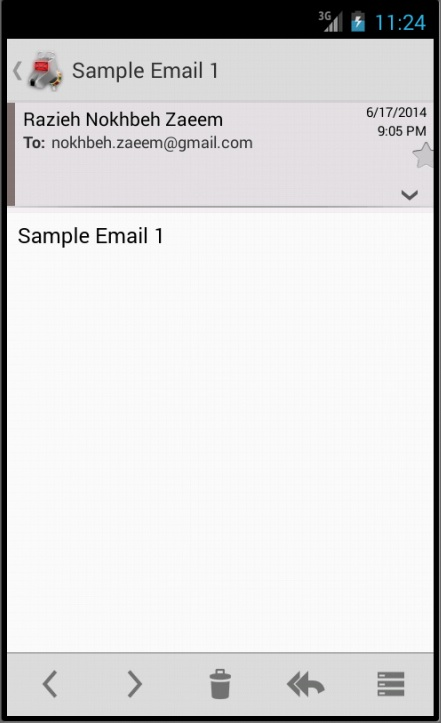
\includegraphics[width=0.225\columnwidth]{figures/bug19/bug19_shot1.jpg}
}
\hfill
\subfloat[A phone call pauses K9Mail.]{
\includegraphics[width=0.225\columnwidth]{figures/bug19/bug19_shot2.jpg}
}
\hfill
\subfloat[K9Mail resumes to the inbox instead of the email.]{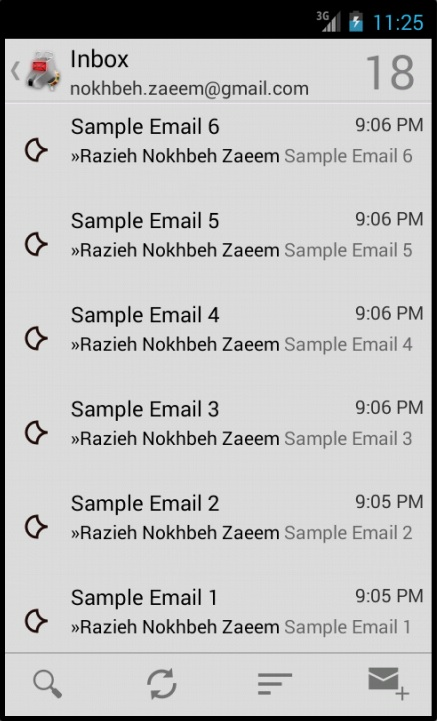
\includegraphics[width=0.225\columnwidth]{figures/bug19/bug19_shot3.jpg}
}
\caption{Pausing and Resuming Bug in K9Mail.}
\label{fig:bug19}
\end{minipage}
\end{figure*}

\indent{\bf Killing and restarting bug in K9Mail}: The operating system decides to kill K9Mail because of low memory while the user is composing an email. K9Mail fails to save the email as a draft, deleting the contents of the email (Figure~\ref{fig:bug17}). We found this bug already reported as issue 161.
\begin{figure*}[!t]
\centering
\begin{minipage}{.8\columnwidth}
%0.225=0.18/0.8
\subfloat[Initially no drafts saved.]{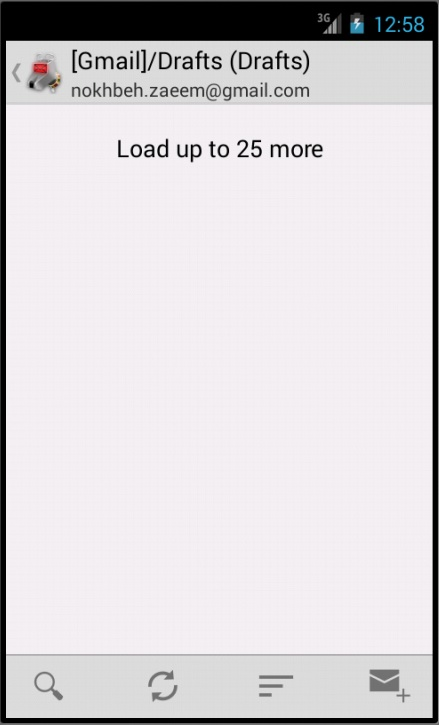
\includegraphics[width=0.225\columnwidth]{figures/bug17/bug17_shot1.jpg}
}
\hfill
\subfloat[While composing an email, the OS kills K9Mail.]{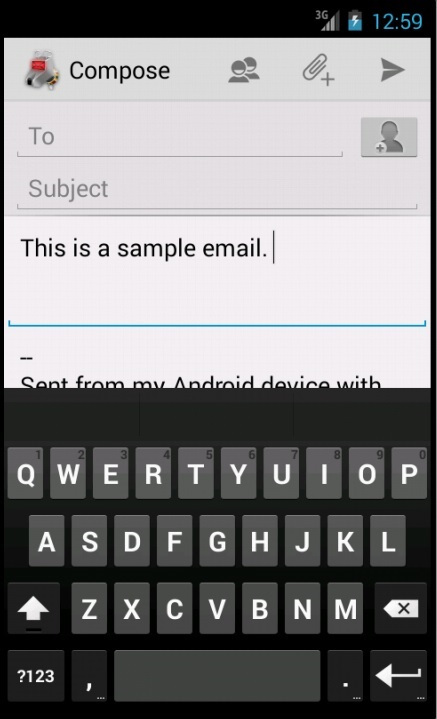
\includegraphics[width=0.225\columnwidth]{figures/bug17/bug17_shot2.jpg}
}
\hfill
\subfloat[K9Mail fails to save a draft.]{
\includegraphics[width=0.225\columnwidth]{figures/bug17/bug17_shot3.jpg}
}
\caption{Killing and Restarting Bug in K9Mail.}
\label{fig:bug17}
\end{minipage}
\end{figure*}

\indent{\bf Rotation bug in Kitchen Timer}: Explained in Section~\ref{example}. We reported this bug as issue 147 to Kitchen Timer.
\\
\indent{\bf Rotation bug in OpenSudoku}: Rotating the device closes the custom pop up for entering numbers and discards them (Figure~\ref{fig:bug25}). We reported this bug as issue 175 to OpenSudoku.
\begin{figure*}[!t]
\centering
\begin{minipage}{.8\columnwidth}
%0.225=0.18/0.8
\subfloat[Before entering numbers.]{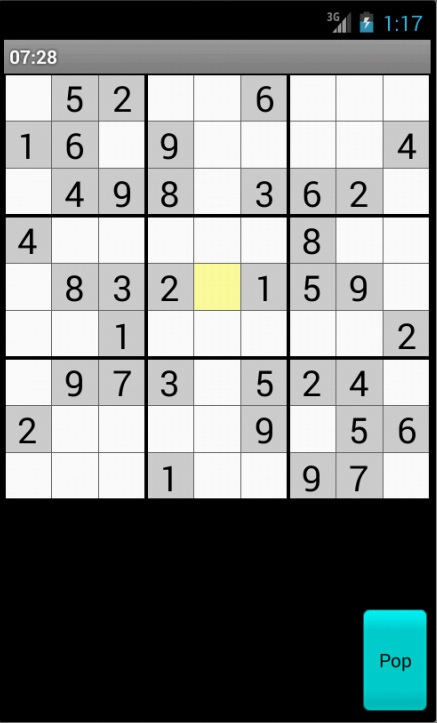
\includegraphics[width=0.225\columnwidth]{figures/bug25/bug25_shot1.jpg}
}
\hfill
\subfloat[Pop up for entering multiple numbers.]{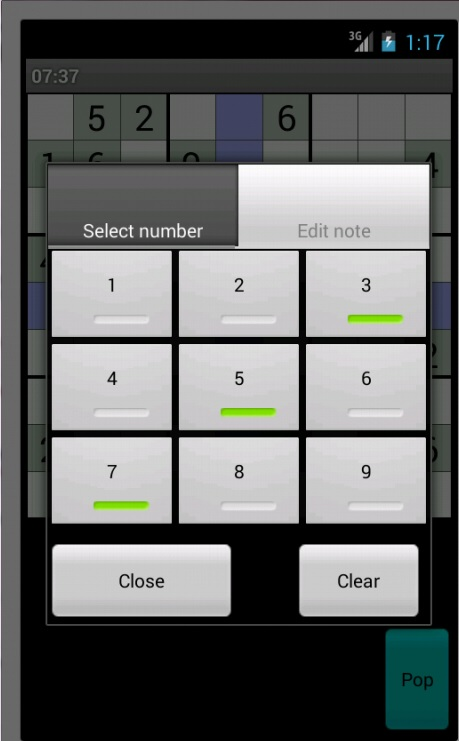
\includegraphics[width=0.225\columnwidth]{figures/bug25/bug25_shot2.jpg}
}
\hfill
\subfloat[Entered numbers discarded after two rotations.]{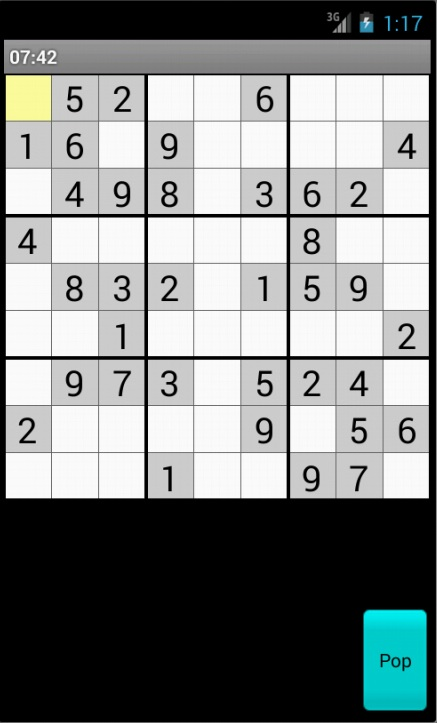
\includegraphics[width=0.225\columnwidth]{figures/bug25/bug25_shot3.jpg}
}
\caption{Rotation Bug in OpenSudoku.}
\label{fig:bug25}
\end{minipage}
\end{figure*}

\indent{\bf Rotation bug in VuDroid}: Rotation clears tab selection. As Figure~\ref{fig:bug9} displays, the default tab is the Browse tab. If the user selects the Recent tab and then rotates the device, the tab selection is rolled back to the default Browse tab. We found this bug already reported and accepted as issue 7.
\begin{figure*}[!t]
\centering
\begin{minipage}{.8\columnwidth}
%0.225=0.18/0.8
\subfloat[Browse is the default tab.]{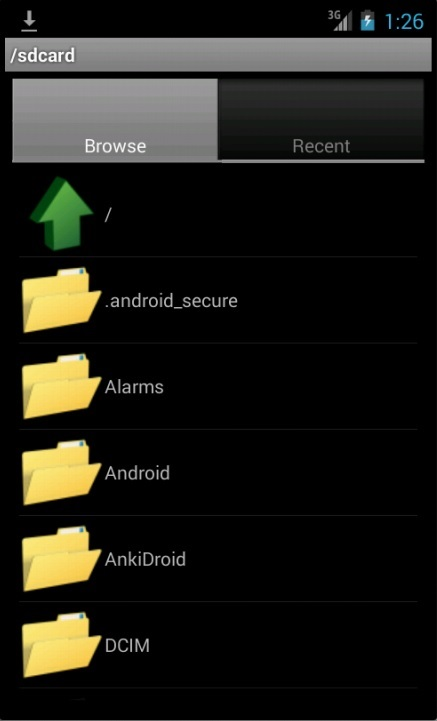
\includegraphics[width=0.225\columnwidth]{figures/bug9/bug9_shot1.jpg}
}
\hfill
\subfloat[Selecting the Recent tab.]{
\includegraphics[width=0.225\columnwidth]{figures/bug9/bug9_shot2.jpg}
}
\hfill
\subfloat[Tab selection cleared after two rotations.]{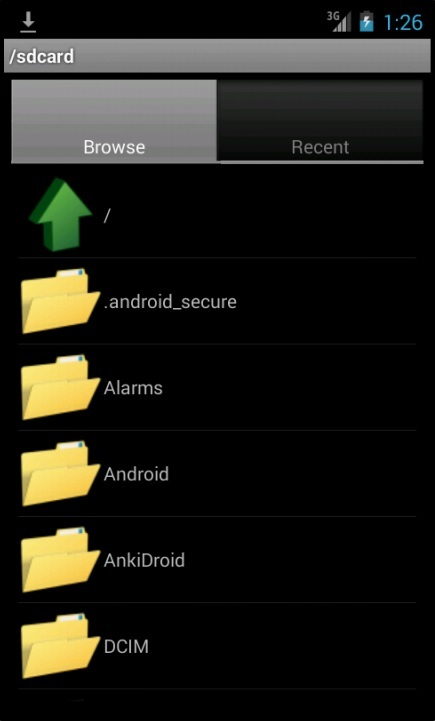
\includegraphics[width=0.225\columnwidth]{figures/bug9/bug9_shot3.jpg}
}
\caption{Rotation Bug in VuDroid.}
\label{fig:bug9}
\end{minipage}
\end{figure*}

\indent{\bf Rotation bug in Nexes Manager}: If there is an empty folder which has no permission (read, write, etc.), rotating the device makes the folder icon disappear (Figure~\ref{fig:bug10}). We reported this bug as issue 9 to Nexes Manager.
\begin{figure*}[!t]
\centering
\begin{minipage}{.5\columnwidth}
%0.36=0.18/0.5
\subfloat[The ``vendor'' folder is empty and has no permission.]{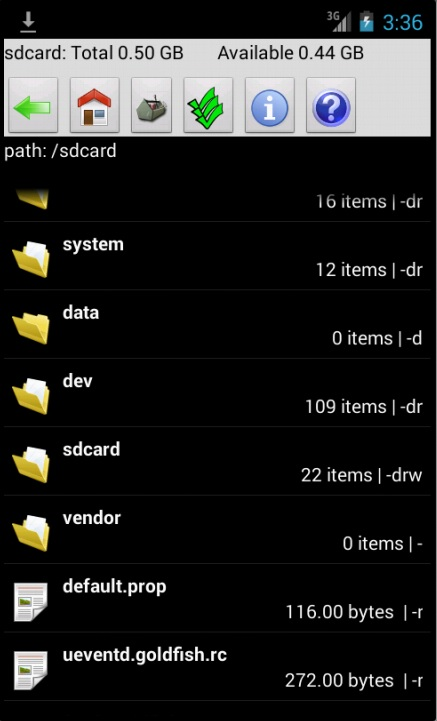
\includegraphics[width=0.36\columnwidth]{figures/bug10/bug10_shot1.jpg}
}
\hfill
\subfloat[The icon beside ``vendor'' disappears after two rotations.]{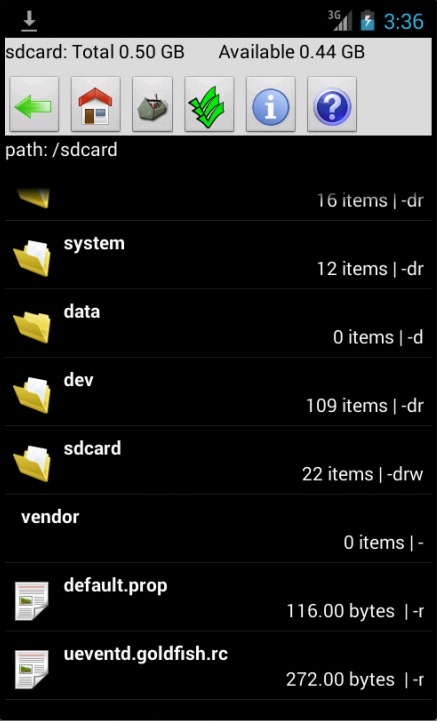
\includegraphics[width=0.36\columnwidth]{figures/bug10/bug10_shot2.jpg}
}
\caption{Rotation Bug in Nexes Manager.}
\label{fig:bug10}
\end{minipage}
\end{figure*}

\indent{\bf Back button bug in Kitchen Timer}: Going to sub-menus and coming back using the hardware Back makes buttons go out of focus. Figure~\ref{fig:bug23} shows how the plus ($+$) button is in focus, but it goes out of focus if the user navigates to the info sub-menu and then comes back using the hardware Back button. We reported this bug as issue 168 to Kitchen Timer.

\begin{figure*}[!t]
\centering
\subfloat[The $+$ button in focus.]{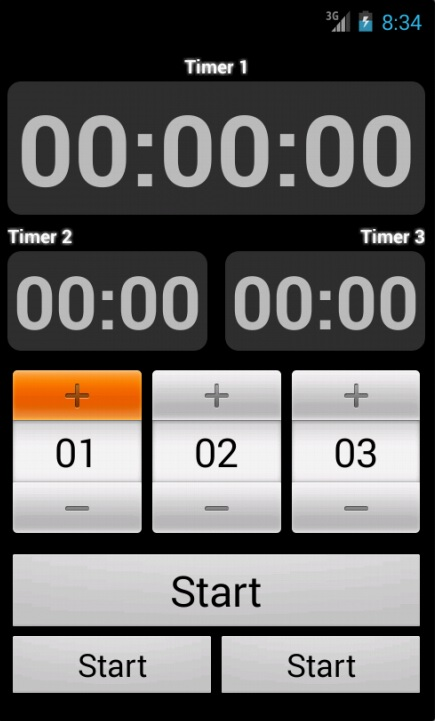
\includegraphics[width=0.18\columnwidth]{figures/bug23/bug23_shot1.jpg}
}
\hfill
\subfloat[Navigating to Menu.]{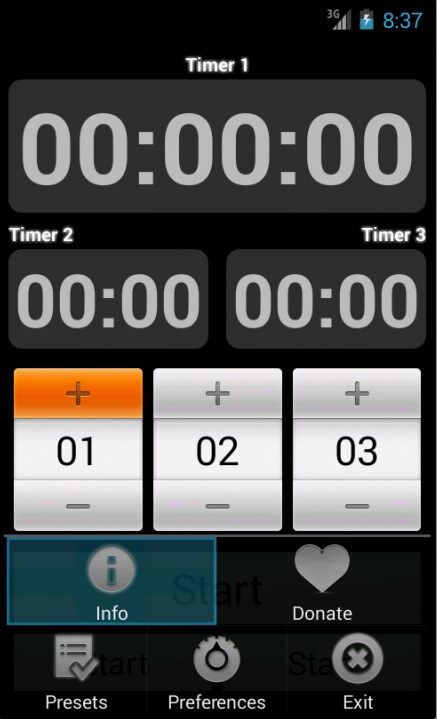
\includegraphics[width=0.18\columnwidth]{figures/bug23/bug23_shot2.jpg}
}
\hfill
\subfloat[Navigating to Menu/Info.]{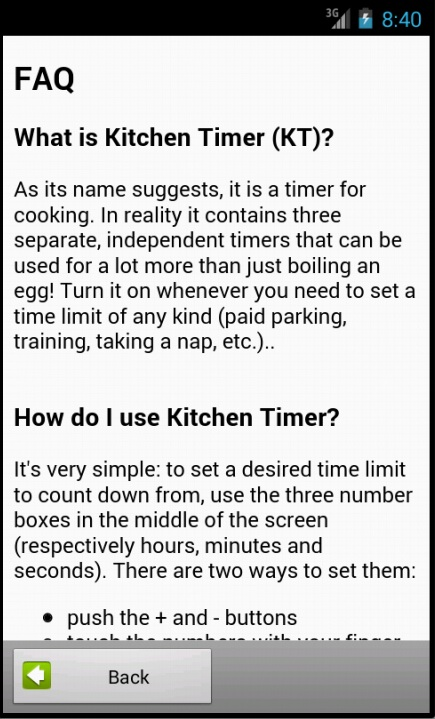
\includegraphics[width=0.18\columnwidth]{figures/bug23/bug23_shot3.jpg}
}
\hfill
\subfloat[Using the hardware Back button. $+$ goes out of focus.]{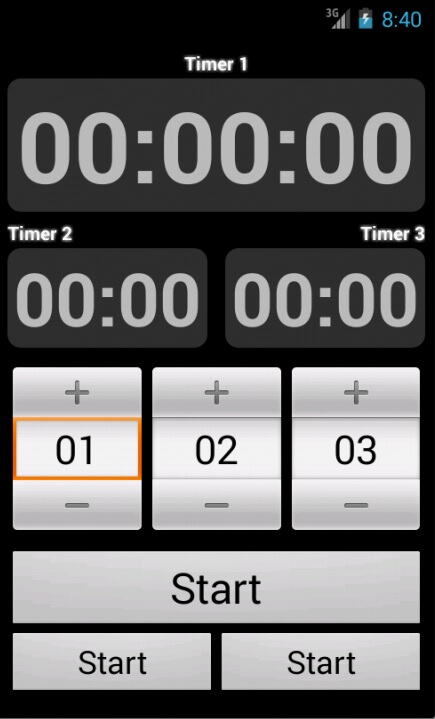
\includegraphics[width=0.18\columnwidth]{figures/bug23/bug23_shot4.jpg}
}
\caption{Back Button Bug in Kitchen Timer.}
\label{fig:bug23}
\end{figure*}

Besides the two bugs that we found already reported in the bug repositories of the corresponding apps, mentioned above as issue 7 of VuDroid and issue 161 of K9Mail, we found another pausing and resuming bug in K9Mail that was independently fixed in version 4.511. All the other \NumBugs{} bugs that \tool{} found were new.
We reported these to the respective developers (e.g., issue 121 of VuDroid, issue 5927 of K9Mail, in addition to the issues listed above) and are awaiting confirmation of the bugs from them. 
%However, we have not yet heard back from developers regarding the reports. 

\tool{} reported a total of $9$ distinct false positives. However, $4$ of these false positives were because of an inconsistency in the Android testing instrumentation, which caused it to act differently when paused programmatically (by tests) or through the emulator GUI (when manually confirming bugs). Another $2$ false positives were because of time sensitivity of some app states. For instance, when a timer is running in Kitchen Timer, rotation changes timer values, not because there is a bug, but rather because the state of a running timer changes with time. Such time sensitivity is usually abstracted out from the app's GUI model to achieve conciseness. Another $2$ false positives manifested because if the app GUI provides a visual back button on the screen, hitting this visual button and then the hardware Back button does not take the app to the original state. The remaining $1$ false positive could be considered a bug, depending on the intent of the app designer.

\subsection{RQ 3: Compactness of Generated Test Suites}
We compared our test generation algorithm to a baseline DFS, in generating test cases that cover all golden edges. For the set of implemented features (rotation, killing and restarting, pausing and resuming, and Back button) we measured the compactness of generated test suites in terms of the number of tests and the cost of the test suite when generated by each of the following algorithms:
%\begin{enumerate}
%\item 
(1) Our basic algorithm;
%\item 
(2) Our algorithm plus the truncation optimization, which truncates test cases after the last golden edge and ignores test cases that do not cover any golden edge;
%\item 
(3) Our algorithm plus the prioritization optimization, which prioritizes golden edges while traversing the model;
%\item 
(4) Our algorithm plus both truncation and prioritization optimizations; and
%\item 
(5) A DFS algorithm starting at the root.
%\end{enumerate}

Table~\ref{table:algoEffectiveness} shows the experimental results. The cost function is calculated with both $\alpha$ and $\beta$ set to 1. As this table shows, our algorithm shows a clear improvement over DFS, in terms of the number of tests as well as the cost of executing test suites. Furthermore, truncation and prioritization improve the results when applied separately (except for Kitchen Timer, for which truncation does not improve the number of tests or cost). In some cases (Notepad, Nexes Manager, and VuDroid), truncation yields better results compared to prioritization, while in the other cases prioritization is more effective. Fortunately, the optimizations are compatible and combinable and using both of them produces even better results for all of the studied apps.

\begin{table}[t!]
\vspace*{-3ex}
\centering
\caption{Compactness of Generated Test Suites.}
\label{table:algoEffectiveness}
{
\begin{tabular}{@{}lr@{}rrr@{}rrr@{}rrr@{}rrr@{}rr@{}}
\toprule
&&\multicolumn{11}{c}{\bf{Our Algorithm}}
&&\multicolumn{2}{c}{\bf{DFS}}\\
&&\multicolumn{2}{c}{\bf{Basic}}
&&\multicolumn{2}{c}{\bf{+ Trunc.}}
&&\multicolumn{2}{c}{\bf{+ Prior.}}
&&\multicolumn{2}{c}{\bf{+ Both}}
\\
\cmidrule{3-4}
\cmidrule{6-7}
\cmidrule{9-10}
\cmidrule{12-13}
\cmidrule{15-16}
\bf{Application}&&\begin{sideways}\bf{\#Tests}\end{sideways}&\begin{sideways}\bf{Cost}\end{sideways}&&\begin{sideways}\bf{\#Tests}\end{sideways}&\begin{sideways}\bf{Cost}\end{sideways}&&\begin{sideways}\bf{\#Tests}\end{sideways}&\begin{sideways}\bf{Cost}\end{sideways}&&\begin{sideways}\bf{\#Tests}\end{sideways}&\begin{sideways}\bf{Cost}\end{sideways}&&\begin{sideways}\bf{\#Tests}\end{sideways}&\begin{sideways}\bf{Cost}\end{sideways}\\
\midrule
\textit{Notepad}&&15&73&&11&59&&12&65&&8&44&&35&114\\
\textit{OpenSudoku}&&13&85&&10&67&&9&67&&7&51&&30&138\\
\textit{Nexes Manager}&&38&200&&24&149&&26&174&&15&127&&97&354\\
\midrule
\textit{VuDroid}&&8&41&&7&38&&7&40&&6&36&&17&57\\
\textit{Kitchen Timer}&&14&113&&14&113&&11&105&&8&75&&70&310\\
\textit{K9Mail}&&30&228&&25&196&&21&187&&16&148&&76&490\\
\bottomrule
\end{tabular}
}
\end{table}


{\bf Threats to Validity}: To minimize threats to internal validity, we automated the entire test generation and execution process and manually identified real bugs from false positives. To address external validity, we experimented with 7 previously studied apps and set forth a criterion to choose 6 other popular apps from open source repositories as discussed in Section~\ref{study}. With respect to construct validity, we strictly followed our traversal algorithm and oracle generation techniques, used well-known frameworks Robotium and JUnit, and manually investigated generated tests for some of the apps. 
One limitation of this work is synthesizing universally applicable oracles, which gives rise to false positives.
General purpose oracles are often either too weak to detect bugs or generate too many false positives. We are mitigating that short-coming by using domain specific knowledge. 

